\section{Observation and Calculations}

Tables I and II show the observed current and voltage values for different filters under the two lighting conditions. The corresponsind plots are shown below. The exponential curves have been fitted with the general equation:
\begin{align}
    I(V) = Ae^{BV} + C
\end{align}

\begin{table*}
    \centering
    \caption{I-V Data for Solar Cell under Incandescent Light}
    \begin{tabular}{|cc|cc|cc|cc|cc|cc|} \hline
    \multicolumn{2}{|c|}{No Filter} & \multicolumn{2}{c|}{Red} & \multicolumn{2}{c|}{Yellow} & \multicolumn{2}{c|}{Magenta} & \multicolumn{2}{c|}{Green} & \multicolumn{2}{c|}{Blue} \\ \hline
    V (V) & I (mA) & V (V) & I (mA) & V (V) & I (mA) & V (V) & I (mA) & V (V) & I (mA) & V (V) & I (mA) \\ \hline
    0.009 & 0.555 & 0.031 & 0.175 & 0.023 & 0.33 & 0.028 & 0.36 & 2.135 & 0.01 & 0.018 & 0.25 \\
    0.097 & 0.554 & 0.136 & 0.174 & 0.124 & 0.33 & 0.314 & 0.36 & 2.165 & 0.01 & 0.121 & 0.25 \\
    0.172 & 0.554 & 0.241 & 0.172 & 0.272 & 0.33 & 0.523 & 0.36 & 1.995 & 0.03 & 0.207 & 0.25 \\
    0.300 & 0.551 & 0.389 & 0.170 & 0.346 & 0.33 & 0.667 & 0.35 & 2.038 & 0.03 & 0.214 & 0.25 \\
    0.581 & 0.548 & 0.518 & 0.167 & 0.462 & 0.33 & 0.952 & 0.34 & 1.906 & 0.04 & 0.386 & 0.25 \\
    0.773 & 0.544 & 0.656 & 0.164 & 0.521 & 0.33 & 1.148 & 0.33 & 1.978 & 0.04 & 0.412 & 0.25 \\
    0.865 & 0.541 & 0.744 & 0.161 & 0.695 & 0.33 & 1.460 & 0.32 & 1.847 & 0.05 & 0.676 & 0.24 \\
    1.067 & 0.532 & 0.822 & 0.158 & 0.749 & 0.32 & 1.811 & 0.28 & 1.887 & 0.05 & 0.922 & 0.23 \\
    1.176 & 0.528 & 0.890 & 0.156 & 0.972 & 0.31 & 1.928 & 0.27 & 1.729 & 0.06 & 1.192 & 0.22 \\
    1.350 & 0.516 & 0.960 & 0.153 & 1.072 & 0.31 & 2.018 & 0.25 & 1.769 & 0.06 & 1.226 & 0.22 \\
    1.452 & 0.508 & 1.064 & 0.149 & 1.161 & 0.31 & 2.029 & 0.25 & 1.791 & 0.06 & 1.326 & 0.22 \\
    1.608 & 0.496 & 1.139 & 0.145 & 1.288 & 0.30 & 2.114 & 0.24 & 1.641 & 0.07 & 1.410 & 0.21 \\
    1.737 & 0.483 & 1.204 & 0.142 & 1.324 & 0.30 & 2.181 & 0.23 & 1.679 & 0.07 & 1.518 & 0.20 \\
    1.792 & 0.476 & 1.302 & 0.136 & 1.427 & 0.29 & 2.263 & 0.22 & 1.491 & 0.08 & 1.815 & 0.18 \\
    1.892 & 0.463 & 1.414 & 0.129 & 1.529 & 0.28 & 2.381 & 0.19 & 1.528 & 0.08 & 2.041 & 0.15 \\
    1.967 & 0.455 & 1.523 & 0.121 & 1.612 & 0.28 & 2.483 & 0.17 & 1.583 & 0.08 & 2.208 & 0.12 \\
    2.043 & 0.443 & 1.610 & 0.114 & 1.652 & 0.27 & 2.573 & 0.15 & 1.346 & 0.09 & 2.376 & 0.09 \\
    2.109 & 0.433 & 1.711 & 0.104 & 1.710 & 0.27 & 2.672 & 0.12 & 1.421 & 0.09 & 2.496 & 0.07 \\
    2.230 & 0.410 & 1.782 & 0.097 & 1.727 & 0.26 & 2.745 & 0.10 & 1.191 & 0.10 & 2.593 & 0.04 \\
    2.290 & 0.394 & 1.841 & 0.091 & 1.846 & 0.25 & 2.831 & 0.07 & 1.229 & 0.10 & 2.695 & 0.01 \\
    2.318 & 0.395 & 1.905 & 0.084 & 1.957 & 0.24 & 2.887 & 0.05 & 1.297 & 0.10 &  &  \\
    2.364 & 0.385 & 1.971 & 0.076 & 2.035 & 0.23 & 2.949 & 0.03 & 1.007 & 0.11 &  &  \\
    2.431 & 0.370 & 2.020 & 0.070 & 2.134 & 0.21 & 2.971 & 0.02 & 1.117 & 0.11 &  &  \\
    2.547 & 0.341 & 2.110 & 0.058 & 2.210 & 0.20 &  &  & 0.750 & 0.12 &  &  \\
    2.645 & 0.310 & 2.167 & 0.050 & 2.325 & 0.18 &  &  & 0.859 & 0.12 &  &  \\
    2.708 & 0.280 & 2.203 & 0.044 & 2.501 & 0.14 &  &  & 0.997 & 0.12 &  &  \\
    2.729 & 0.273 & 2.241 & 0.038 & 2.619 & 0.11 &  &  & 0.250 & 0.13 &  &  \\
    2.772 & 0.260 & 2.274 & 0.032 & 2.715 & 0.08 &  &  & 0.474 & 0.13 &  &  \\
    2.829 & 0.241 & 2.306 & 0.027 & 2.784 & 0.06 &  &  & 0.637 & 0.13 &  &  \\
    2.860 & 0.229 & 2.323 & 0.023 & 2.866 & 0.03 &  &  & 0.009 & 0.14 &  &  \\
    2.905 & 0.211 &  &  & 2.909 & 0.02 &  &  & 0.107 & 0.14 &  &  \\
    2.958 & 0.190 &  &  & 2.910 & 0.00 &  &  &  &  &  &  \\
    % 3.000 & 0.172 &  &  &  &  &  &  &  &  &  &  \\
    3.023 & 0.161 &  &  &  &  &  &  &  &  &  &  \\
    % 3.047 & 0.150 &  &  &  &  &  &  &  &  &  &  \\
    3.070 & 0.140 &  &  &  &  &  &  &  &  &  &  \\
    % 3.091 & 0.130 &  &  &  &  &  &  &  &  &  &  \\
    3.112 & 0.119 &  &  &  &  &  &  &  &  &  &  \\
    3.127 & 0.111 &  &  &  &  &  &  &  &  &  &  \\
    % 3.160 & 0.092 &  &  &  &  &  &  &  &  &  &  \\
    % 3.171 & 0.087 &  &  &  &  &  &  &  &  &  &  \\
    % 3.180 & 0.081 &  &  &  &  &  &  &  &  &  &  \\
    % 3.190 & 0.074 &  &  &  &  &  &  &  &  &  &  \\
    3.196 & 0.070 &  &  &  &  &  &  &  &  &  &  \\
    3.212 & 0.060 &  &  &  &  &  &  &  &  &  &  \\
    3.240 & 0.042 &  &  &  &  &  &  &  &  &  &  \\
    3.257 & 0.032 &  &  &  &  &  &  &  &  &  & \\ \hline
    \end{tabular}
    \label{tab:in}
\end{table*}
\begin{table*}
    \centering
    \caption{I-V Data for Solar Cell under Sunlight}
    \begin{tabular}{|cc|cc|cc|cc|cc|cc|} \hline
    \multicolumn{2}{|c|}{No Filter} & \multicolumn{2}{c|}{Red} & \multicolumn{2}{c|}{Yellow} & \multicolumn{2}{c|}{Magenta} & \multicolumn{2}{c|}{Green} & \multicolumn{2}{c|}{Blue} \\ \hline
    V (V) & I (mA) & V (V) & I (mA) & V (V) & I (mA) & V (V) & I (mA) & V (V) & I (mA) & V (V) & I (mA) \\ \hline
    0.254 & 77.10 & 0.286 & 52.61 & 0.391 & 77.10 & 0.181 & 31.38 & 0.190 & 37.35 & 0.231 & 43.41 \\
    0.781 & 76.10 & 0.781 & 44.31 & 1.771 & 76.10 & 0.982 & 28.38 & 1.400 & 36.53 & 0.572 & 43.01 \\
    2.548 & 73.10 & 1.361 & 38.72 & 4.122 & 73.10 & 2.132 & 26.89 & 4.426 & 33.72 & 1.841 & 42.61 \\
    4.895 & 63.10 & 2.861 & 33.81 & 4.724 & 63.10 & 4.215 & 24.69 & 4.819 & 26.60 & 4.508 & 40.98 \\
    5.276 & 57.55 & 4.312 & 30.87 & 4.931 & 55.80 & 4.591 & 22.19 & 4.910 & 23.10 & 4.689 & 38.76 \\
    5.405 & 49.32 & 4.500 & 27.20 & 4.982 & 53.43 & 4.612 & 19.78 & 4.912 & 21.99 & 4.821 & 35.68 \\
    5.421 & 45.86 & 4.669 & 23.18 & 5.032 & 48.54 & 4.782 & 17.72 & 4.956 & 19.93 & 4.936 & 31.79 \\
    5.441 & 43.35 & 4.697 & 20.21 & 5.098 & 41.24 & 4.853 & 15.24 & 4.995 & 17.93 & 4.983 & 29.86 \\
    5.444 & 40.67 & 4.845 & 17.61 & 5.180 & 37.75 & 4.905 & 13.40 & 5.015 & 16.56 & 5.052 & 26.03 \\
    5.492 & 33.09 & 4.880 & 15.90 & 5.222 & 32.34 & 4.939 & 12.30 & 5.038 & 15.29 & 5.081 & 24.77 \\
    5.494 & 38.81 & 4.870 & 15.87 & 5.237 & 31.38 & 4.922 & 10.35 & 5.050 & 14.72 & 5.139 & 22.36 \\
    5.497 & 28.72 & 4.933 & 14.23 & 5.251 & 29.42 & 5.008 & 9.45 & 5.086 & 13.91 & 5.164 & 20.35 \\
    5.502 & 36.71 & 4.969 & 12.47 & 5.263 & 27.25 & 5.019 & 8.70 & 5.093 & 12.86 & 5.197 & 17.68 \\
    5.506 & 34.98 & 4.999 & 10.67 & 5.279 & 24.92 & 5.033 & 7.68 & 5.116 & 11.47 & 5.220 & 16.09 \\
    5.511 & 26.78 & 4.979 & 9.60 & 5.302 & 22.63 & 5.057 & 6.70 & 5.121 & 10.57 & 5.237 & 14.45 \\
    5.517 & 23.12 & 5.030 & 8.00 & 5.319 & 20.29 & 5.041 & 6.38 & 5.144 & 8.76 & 5.243 & 13.13 \\
    5.528 & 31.68 & 5.041 & 6.23 & 5.325 & 18.55 & 5.064 & 6.00 & 5.169 & 7.57 & 5.258 & 12.42 \\
    5.540 & 19.27 & 5.058 & 5.23 & 5.333 & 17.09 & 5.068 & 5.04 & 5.173 & 6.98 & 5.265 & 11.13 \\
    5.549 & 18.86 & 5.091 & 4.28 & 5.330 & 16.53 & 5.086 & 4.39 & 5.235 & 3.68 & 5.275 & 10.43 \\
    5.580 & 15.61 & 5.104 & 3.44 & 5.334 & 15.18 & 5.092 & 3.85 & 5.240 & 3.20 & 5.281 & 9.56 \\
    5.588 & 13.53 & 5.128 & 1.00 & 5.342 & 13.84 & 5.103 & 3.42 & 5.279 & 2.94 & 5.301 & 8.68 \\
    5.594 & 11.93 &  &  & 5.344 & 12.89 & 5.111 & 2.85 & 5.300 & 1.07 & 5.298 & 7.15 \\
    5.598 & 10.82 &  &  & 5.351 & 11.74 & 5.124 & 2.29 & 5.309 & 1.03 & 5.300 & 6.43 \\
    5.606 & 7.25 &  &  & 5.356 & 10.81 & 5.125 & 1.82 &  &  & 5.276 & 5.81 \\
    5.617 & 5.18 &  &  & 5.354 & 9.68 & 5.151 & 1.00 &  &  & 5.291 & 4.06 \\
    5.630 & 2.55 &  &  & 5.356 & 7.97 &  &  &  &  & 5.296 & 2.82 \\
    5.633 & 0.15 &  &  & 5.355 & 7.05 &  &  &  &  & 5.292 & 2.03 \\
    5.634 & 1.93 &  &  & 5.351 & 6.51 &  &  &  &  & 5.296 & 1.29 \\
    5.638 & 1.30 &  &  & 5.347 & 5.85 &  &  &  &  &  &  \\
    5.639 & 1.00 &  &  & 5.355 & 3.46 &  &  &  &  &  &  \\
    5.639 & 0.62 &  &  & 5.348 & 1.64 &  &  &  &  &  &  \\
    5.641 & 0.04 &  &  & 5.369 & 1.04 &  &  &  &  &  &  \\ \hline
    \end{tabular}
    \label{tab:in}
\end{table*}

\subsection{Under Incandescent Lamp}

\subsubsection{No Filter}
\begin{itemize}
    \item $V_\text{mp} = 2.318$ V and $I_\text{mp} = 0.395$ mA
    \item Max. Power ($P_\text{max}$) $= 0.916 \pm 0.023 $ mW
    \item Short Circuit Current ($I_\text{sc}$) $= 0.555 \pm 0.001$ mA
    \item Open Circuit Voltage ($V_\text{oc}$) $= 3.257 \pm 0.001$ V
    \item Fill Factor $= 0.507 \pm 0.016$
\end{itemize}

\begin{figure}[H]
    \centering
    \includegraphics[width=1\columnwidth]{images/in/no.eps}
    \caption{I-V and P-V curves for the solar cell with no filter indoors}
\end{figure}

% -----------

\subsubsection{Red Filter}
\begin{itemize}
    \item $V_\text{mp} = 1.523$ V and $I_\text{mp} = 0.121$ mA
    \item Max. Power ($P_\text{max}$) $= 0.184 \pm 0.015 $ mW
    \item Short Circuit Current ($I_\text{sc}$) $= 0.175 \pm 0.001$ mA
    \item Open Circuit Voltage ($V_\text{oc}$) $= 2.323 \pm 0.001$ V
    \item Fill Factor $= 0.453 \pm 0.046$
\end{itemize}

\begin{figure}[H]
    \centering
    \includegraphics[width=1\columnwidth]{images/in/red.eps}
    \caption{I-V and P-V curves for the solar cell with red filter indoors}
\end{figure}

% -----------

\subsubsection{Blue Filter}
\begin{itemize}
    \item $V_\text{mp} = 1.815$ V and $I_\text{mp} = 0.18$ mA
    \item Max. Power ($P_\text{max}$) $= 0.327 \pm 0.018 $ mW
    \item Short Circuit Current ($I_\text{sc}$) $= 0.25 \pm 0.01$ mA
    \item Open Circuit Voltage ($V_\text{oc}$) $= 2.695 \pm 0.001$ V
    \item Fill Factor $= 0.485 \pm 0.033$
\end{itemize}

\begin{figure}[H]
    \centering
    \includegraphics[width=1\columnwidth]{images/in/blue.eps}
    \caption{I-V and P-V curves for the solar cell with blue filter indoors}
\end{figure}

% -----------

\subsubsection{Green Filter}
\begin{itemize}
    \item $V_\text{mp} = 1.297$ V and $I_\text{mp} = 0.10$ mA
    \item Max. Power ($P_\text{max}$) $= 0.130 \pm 0.013 $ mW
    \item Short Circuit Current ($I_\text{sc}$) $= 0.14 \pm 0.01$ mA
    \item Open Circuit Voltage ($V_\text{oc}$) $= 2.165 \pm 0.001$ V
    \item Fill Factor $= 0.428 \pm 0.053$
\end{itemize}

\begin{figure}[H]
    \centering
    \includegraphics[width=1\columnwidth]{images/in/green.eps}
    \caption{I-V and P-V curves for the solar cell with green filter indoors}
\end{figure}

% -----------

\subsubsection{Magenta Filter}
\begin{itemize}
    \item $V_\text{mp} = 1.928$ V and $I_\text{mp} = 0.27$ mA
    \item Max. Power ($P_\text{max}$) $= 0.521 \pm 0.019 $ mW
    \item Short Circuit Current ($I_\text{sc}$) $= 0.36 \pm 0.01$ mA
    \item Open Circuit Voltage ($V_\text{oc}$) $= 2.971 \pm 0.001$ V
    \item Fill Factor $= 0.487 \pm 0.023$
\end{itemize}

\begin{figure}[H]
    \centering
    \includegraphics[width=1\columnwidth]{images/in/pink.eps}
    \caption{I-V and P-V curves for the solar cell with magenta filter indoors}
\end{figure}


% -----------
\subsubsection{Yellow Filter}
\begin{itemize}
    \item $V_\text{mp} = 1.957$ V and $I_\text{mp} = 0.24$ mA
    \item Max. Power ($P_\text{max}$) $= 0.470 \pm 0.020 $ mW
    \item Short Circuit Current ($I_\text{sc}$) $= 0.33 \pm 0.01$ mA
    \item Open Circuit Voltage ($V_\text{oc}$) $= 2.91 \pm 0.01$ V
    \item Fill Factor $= 0.489 \pm 0.025$
\end{itemize}

\begin{figure}[H]
    \centering
    \includegraphics[width=1\columnwidth]{images/in/yellow.eps}
    \caption{I-V and P-V curves for the solar cell with yellow filter indoors}
\end{figure}

% --------------
% --------------

\subsection{Under Sunlight}

\subsubsection{No Filter}
\begin{itemize}
    \item $V_\text{mp} = 4.895$ V and $I_\text{mp} = 63.1$ mA
    \item Max. Power ($P_\text{max}$) $= 308.874 \pm 0.080 $ mW
    \item Short Circuit Current ($I_\text{sc}$) $= 77.10 \pm 0.01$ mA
    \item Open Circuit Voltage ($V_\text{oc}$) $= 5.641 \pm 0.001$ V
    \item Fill Factor $= 0.710 \pm 0.001$
\end{itemize}

\begin{figure}[H]
    \centering
    \includegraphics[width=1\columnwidth]{images/out/no.eps}
    \caption{I-V and P-V curves for the solar cell with no filter outdoors}
\end{figure}

% -----------

\subsubsection{Red Filter}
\begin{itemize}
    \item $V_\text{mp} = 4.312$ V and $I_\text{mp} = 30.87$ mA
    \item Max. Power ($P_\text{max}$) $= 133.111 \pm 0.053 $ mW
    \item Short Circuit Current ($I_\text{sc}$) $= 52.61 \pm 0.01$ mA
    \item Open Circuit Voltage ($V_\text{oc}$) $= 5.128 \pm 0.001$ V
    \item Fill Factor $= 0.493 \pm 0.001$
\end{itemize}

\begin{figure}[H]
    \centering
    \includegraphics[width=1\columnwidth]{images/out/red.eps}
    \caption{I-V and P-V curves for the solar cell with red filter outdoors}
\end{figure}

% % -----------

\subsubsection{Blue Filter}
\begin{itemize}
    \item $V_\text{mp} = 4.508$ V and $I_\text{mp} = 40.98$ mA
    \item Max. Power ($P_\text{max}$) $= 184.738 \pm 0.061 $ mW
    \item Short Circuit Current ($I_\text{sc}$) $= 43.41 \pm 0.01$ mA
    \item Open Circuit Voltage ($V_\text{oc}$) $= 5.301 \pm 0.001$ V
    \item Fill Factor $= 0.803 \pm 0.001$
\end{itemize}

\begin{figure}[H]
    \centering
    \includegraphics[width=1\columnwidth]{images/out/blue.eps}
    \caption{I-V and P-V curves for the solar cell with blue filter outdoors}
\end{figure}

% % -----------

\subsubsection{Green Filter}
\begin{itemize}
    \item $V_\text{mp} = 4.426$ V and $I_\text{mp} = 33.72$ mA
    \item Max. Power ($P_\text{max}$) $= 149.245 \pm 0.056 $ mW
    \item Short Circuit Current ($I_\text{sc}$) $= 37.35 \pm 0.01$ mA
    \item Open Circuit Voltage ($V_\text{oc}$) $= 5.309 \pm 0.001$ V
    \item Fill Factor $= 0.753 \pm 0.001$
\end{itemize}

\begin{figure}[H]
    \centering
    \includegraphics[width=1\columnwidth]{images/out/green.eps}
    \caption{I-V and P-V curves for the solar cell with green filter outdoors}
\end{figure}

% % -----------

\subsubsection{Magenta Filter}
\begin{itemize}
    \item $V_\text{mp} = 4.215$ V and $I_\text{mp} = 24.69$ mA
    \item Max. Power ($P_\text{max}$) $= 104.068 \pm 0.049 $ mW
    \item Short Circuit Current ($I_\text{sc}$) $= 31.38 \pm 0.01$ mA
    \item Open Circuit Voltage ($V_\text{oc}$) $= 5.151 \pm 0.001$ V
    \item Fill Factor $= 0.644 \pm 0.001$
\end{itemize}

\begin{figure}[H]
    \centering
    \includegraphics[width=1\columnwidth]{images/out/pink.eps}
    \caption{I-V and P-V curves for the solar cell with magenta filter outdoors}
\end{figure}


% % -----------
\subsubsection{Yellow Filter}
\begin{itemize}
    \item $V_\text{mp} = 4.122$ V and $I_\text{mp} = 73.1$ mA
    \item Max. Power ($P_\text{max}$) $= 301.318 \pm 0.084 $ mW
    \item Short Circuit Current ($I_\text{sc}$) $= 77.10 \pm 0.01$ mA
    \item Open Circuit Voltage ($V_\text{oc}$) $= 5.369 \pm 0.001$ V
    \item Fill Factor $= 0.728 \pm 0.001$
\end{itemize}

\begin{figure}[H]
    \centering
    \includegraphics[width=1\columnwidth]{images/out/yellow.eps}
    \caption{I-V and P-V curves for the solar cell with yellow filter outdoors}
\end{figure}

% --------------
% --------------

A summary of all the parameters are shown below in Tables III and IV.\\

\begin{table}[H]
    \centering
    \begin{tabular}{|c|c|c|c|c|}
    \hline
    Filter & $P_\text{max}$ & $V_\text{oc}$ & $I_\text{sc}$ & FF \\
     & (mW) & (V) & (mA) &  \\ \hline   
    No Filter & 0.916 $\pm$ 0.023 & 3.257 & 0.555 & 0.507 $\pm$ 0.016\\ 
    Red & 0.184 $\pm$ 0.015 & 2.323 & 0.175 & 0.453 $\pm$ 0.046\\ 
    Yellow & 0.470 $\pm$ 0.020 & 2.910 & 0.33 & 0.489 $\pm$ 0.025\\ 
    Magenta & 0.521 $\pm$ 0.019 & 2.971 & 0.36 & 0.487 $\pm$ 0.023\\ 
    Green & 0.130 $\pm$ 0.013 & 2.165 & 0.14 & 0.428 $\pm$ 0.053\\ 
    Blue & 0.327 $\pm$ 0.018 & 2.695 & 0.25 & 0.485 $\pm$ 0.033\\ \hline
    \end{tabular}
    \caption{Open-circuit voltage, short-circuit current,
    maximum power output, and Fill Factor for the solar
    cell under incandescent lamp}
    \label{in_all}
\end{table}
\begin{table}[H]
    \centering
    \begin{tabular}{|c|c|c|c|c|}
    \hline
    Filter & $P_\text{max}$ & $V_\text{oc}$ & $I_\text{sc}$ & FF \\
     & (mW) & (V) & (mA) &  \\ \hline   
    No Filter & 308.874 $\pm$ 0.080 & 5.641 & 77.1 & 0.701 $\pm$ 0.001 \\ 
    Red & 133.111 $\pm$ 0.053 & 5.128 & 52.61 & 0.493 $\pm$ 0.001\\ 
    Yellow & 301.318 $\pm$ 0.084 & 5.369 & 77.10 & 0.728 $\pm$ 0.001\\ 
    Magenta & 104.068 $\pm$ 0.049 & 5.151 & 31.38 & 0.644 $\pm$ 0.001\\ 
    Green & 149.245 $\pm$ 0.056 & 5.309 & 37.35 & 0.753 $\pm$ 0.001\\ 
    Blue & 184.738 $\pm$ 0.061 & 5.301 & 43.41 & 0.803 $\pm$ 0.001\\ \hline
    \end{tabular}
    \caption{Open-circuit voltage, short-circuit current,
    maximum power output, and Fill Factor for the solar
    cell under sunlight}
    \label{out_all}
\end{table}

Below are the comparative plots for I-V and P-V with different filters.

\begin{figure}[H]
    % \begin{subfigure}{\linewidth}
        \centering
        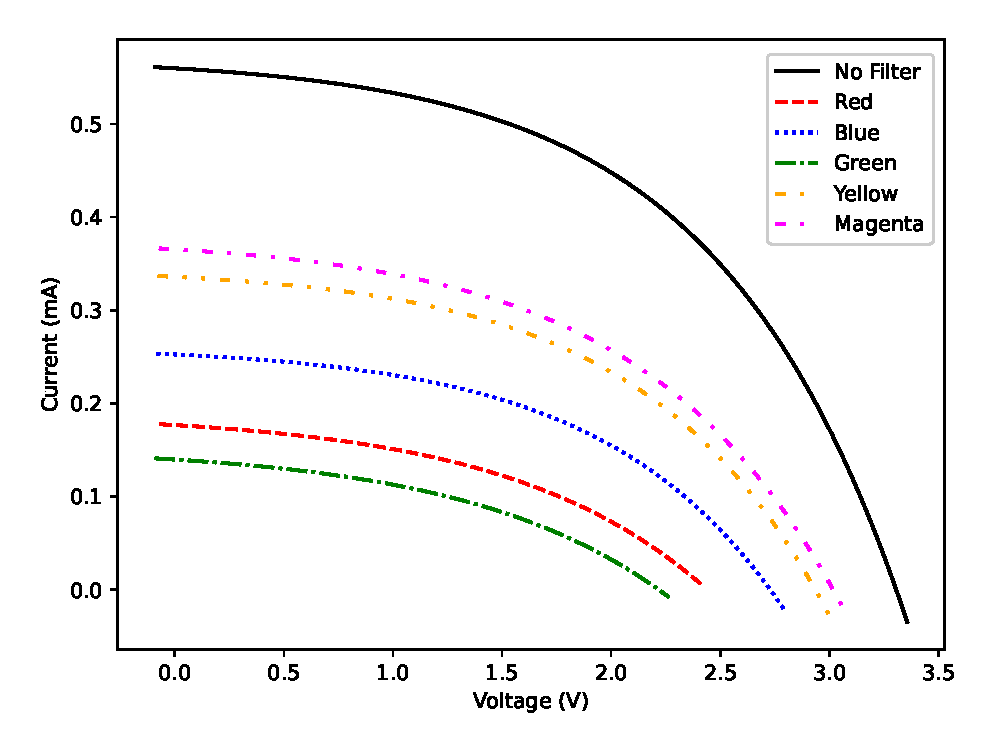
\includegraphics[width=1\columnwidth]{images/in/iv.eps}
        % \caption{}
    % \end{subfigure}
    \caption{I-V curves for the solar cell with different filters under incandescent lamp}
\end{figure}

\begin{figure}
    % \ContinuedFloat
    % \begin{subfigure}{\linewidth}
        \centering
        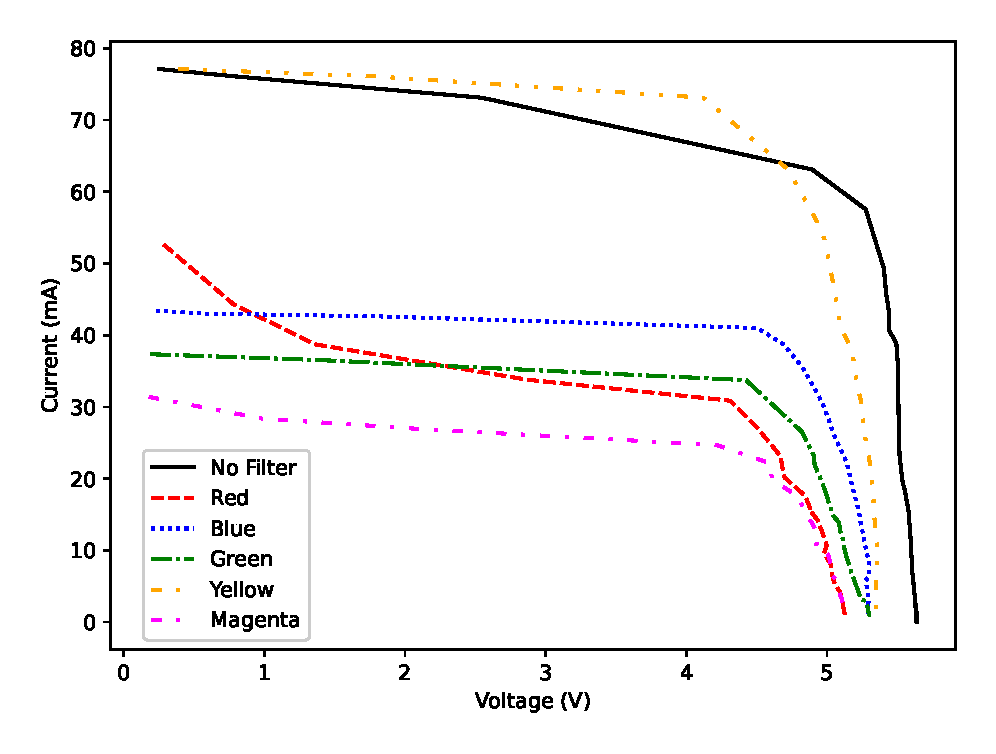
\includegraphics[width=1\columnwidth]{images/out/iv.eps}
        % \caption{U}
    % \end{subfigure}
    \caption{I-V curves for the solar cell with different filters under sunlight}
\end{figure}

\begin{figure}
    \centering
    \includegraphics[width=1\columnwidth]{images/in/powers.eps}
    \caption{P-V curves for the solar cell with different filters under incandescent lamp}
\end{figure}

\begin{figure}
    \centering
    \includegraphics[width=1\columnwidth]{images/out/powers.eps}
    \caption{P-V curves for the solar cell with different filters under sunlight}
\end{figure}
